\section{Introduction}

In many applications data can be represented as a matrix that defines a mapping between two feature spaces. As an example a dataset of ratings of users for movies may be considered. As depicted in Figure~\ref{fig:exmpl_matrix}, such a dataset can be modeled as a matrix in which each row represents a user, each column a movie, and each value a rating that a user has given a movie . 

\begin{figure}[h]
\centering
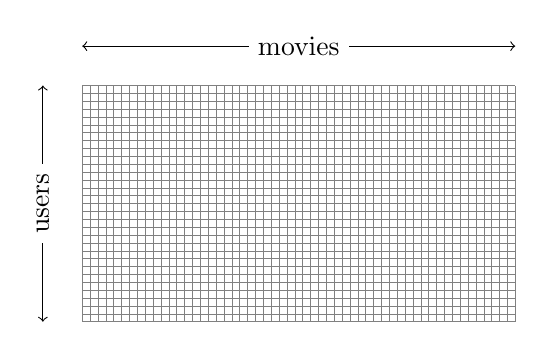
\begin{tikzpicture}
\draw[<->] (0,0.5) -- (0,3.5) node[pos=.5,sloped,fill=white] {users};
\draw[<->] (0.5,4) -- (6,4) node[pos=.5,sloped,fill=white] {movies};
%\draw      (0.5,0.5)  rectangle(6,3.5);
\draw[step=1mm,gray,very thin] (0.4999,0.4999) grid (6,3.5);
\end{tikzpicture}
\caption{Example of a matrix that represents a dataset containing ratings from users for movies}
\label{fig:exmpl_matrix}
\end{figure}

The general goal of such a matrix or vector representation of data is to exploit well known mathematical functions and properties to process the data, which is done by many machine learning and data mining algorithms. However, if at least one feature space is very large, which means in the example that the number of movies or users is very high, the practical application of this approach is hindered. The most obvious reason for this roots in the size of the data, that can get too large as to fit into main memory or as to be processed efficiently. Beyond that a large number of (possibly dependent) dimensions can render mathematical functions useless---especially vector distances, on which important algorithms in machine learning and data mining rely. The latter class of phenomena is grouped under the term \textsl{curse of dimensionality}.

One approach to tackle the aforementioned problems is to reduce or compress the size or number of dimensions of the data's feature spaces. In the example, this would mean to compress a number of movies to a more abstract concept like i.e. genres. 

%Another example for this approach is a dataset that contains for a corpus of documents and a dictionary of words the number of how often a word appears in a document. A matrix representation of this situation models i.e. documents as rows, columns as words, and values as the sum of how often a word appears in a document.

